\chapter{A Quark Picture of Hadrons} \label{chap::QM}

The Quark Model was conceived in the mid-sixties as a classification scheme for the veritable zoo of hadrons which had been discovered (e.g. $\pi, K,p,n,\Lambda,\Sigma,\Xi$) . If one assumed the existence of three elementary particles, called quarks, the masses of experimentally observed states could be organized into specific patterns based on the different ways of combining the quarks\footnote{We will use the term \emph{valence quarks} to describe the minimal number of quarks necessary to construct the spin, flavor, parity, and charge conjugation quantum numbers of hadrons. These are to be distinguished from \emph{constituent quarks} which refer to the dressed or massive quarks used in model calculations. In the simple picture we consider the constituent quarks are also the valence quarks.}. This was an extremely powerful realization. It yielded a theoretical prediction of the existence and mass of the $\Omega^-$ baryon in 1962. Eventual observation of this baryon in 1963 at Brookhaven National Laboratory confirmed suspicions about the existence of quarks, resulted in a Nobel Prize for Murray Gell-Mann, and was an important milestone on the road that led to the discovery of the theory of Quantum Chromodynamics.  

A more modern understanding of QCD tells us that the hadrons are actually strongly interacting admixtures of quarks and gluons, the fundamental fields of the theory.  While we know that valence quarks are an approximation, it turns out to be a quite useful one. 

Quantum Chromodynamics is an asymptotically free Quantum Field Theory. This means that at small distance scales the coupling, which can be thought of as describing the strength of quark-glue and glue-glue interactions, is small. At larger distance scales the coupling takes on a larger value and the theory is said to be confining\footnote{Here a large distance scale can be roughly thought of as $0.1\mathrm{fm} = 10^{-16}\mathrm{m}$, about a tenth of the size of a typical hadron.}. We cannot directly observe the fundamental quark and gluon fields (as opposed to the electrons and photons of Quantum Electrodynamics), rather we only have access to the hadronic excitations of the theory. 

The Quark Model takes advantage of the confining nature of QCD, organizing the hadrons into patterns of multiplets based on the purported existence of constituent quarks corresponding to the up, down, and strange flavor quarks present in the standard model. Effectively we add a minimal number of constituent quarks together to form the valence structure of the hadron. 

 As an example we can consider a simple baryon; generically we think of these objects as being composed of three valance quarks, bound in a potential of gluonic origin, which gives rise to the hadronic states we observe in nature such as protons and neutrons. Although we know that the Quark Model lacks a fundamental feature of the actual gauge theory (the gluons), the valence quark picture yields an extremely effective classification scheme still in use today.

Colloquially we use the term Quark Model as a catch-all phrase for calculations and models which feature quarks without explicitly including the gauge degrees of freedom occurring in QCD. 

In this chapter we introduce some background material pertaining to Quark Models focusing in particular on mesons, hadrons which can be thought of as quark anti-quark pairs. In \secref{QM::CQM} we demonstrate the construction of $q\bar{q}$ states finding that this construction produces a spectrum of allowed states with no support for a subset of quantum numbers which are generically referred to as exotic and are one of the main focuses of this manuscript. 


%%%%%%%%%%%%%%%%%%%%%%%%%%%%%%%%%%%%%%%%%%%%%%%%%%%%%%%%%
%%%%%%%%%%%%%%%%%%%%%%%%%%%%%%%%%%%%%%%%%%%%%%%%%%%%%%%%%
%%%%%%%%%%%%%%%%%%%%%%%%%%%%%%%%%%%%%%%%%%%%%%%%%%%%%%%%%

\section{Quarkonia Multiplets} \label{QM::CQM}

One starting point for quark model calculations is the realization that the bulk properties of the experimentally observed hadronic spectrum appears to favor an interpretation of hadrons as combinations of $\mathcal{O}(300\mathrm{MeV})$ \emph{constituent} quarks. Equivalently, the degrees of freedom manifest in the experimental spectrum appear to be constituent quarks as opposed to the nearly massless quarks featuring in the QCD Lagrangian. Assuming for the moment that constituent quarks do appear as effective degrees of freedom within QCD we illustrate some well known phenomenology related to quark anti-quark angular wave functions. 

By making the approximation that mesons are bound states made up of one quark and one antiquark  we will find that we can derive the allowed $J^{PC}$ (spin, parity, charge-conjugation) quantum numbers. We will specialize to a non-relativistic theory in which there is a single heavy flavor and work under the assumption that the potential between the quarks is central. 

%The generic starting point for a quark model calculation is the approximation that hadrons can be regarded as simple bound states of the ``valance quark content'' which give rise to the quantum numbers of the hadron.  Here we will specialize to a fictitious world in which there is a single flavor heavy quark. We are working under the assumption that the potential between the quarks is central. 

%%%%%%%%%%%%%%%%%%%%%%%%%%%%%%%%%%%%%%%%%%%%%%%%%%%%%%%%%
%%%%%%%%%%%%%%%%%%%%%%%%%%%%%%%%%%%%%%%%%%%%%%%%%%%%%%%%%
%%%%%%%%%%%%%%%%%%%%%%%%%%%%%%%%%%%%%%%%%%%%%%%%%%%%%%%%%
\subsection{Construction of Meson Wavefunctions}
%{\color{blue} Derive something slicker here, start from ladder operators?}

The construction of wavefunctions is easiest in momentum space. Working in the center of momentum frame we can generically decompose the wave-function into a radial momentum space wave-function, $\phi$, multiplying a spherical harmonic.  In order to construct a state of total angular momentum, $J$, we first couple the quark spins together ($S=0,1$) and then add in any additional angular momentum from the spherical harmonic ($L=0,1,2,\ldots$). The generic form of the wave-function for the $n$'th radial quantum number is: 
\begin{align*}
| n^{2S+1}L_J , m_J \rangle_{q\bar{q}} =   &\sum_{m_L, m_s} \langle L m_L; S m_s | J m_J \rangle \sum_{r,\bar{r}} \langle \tfrac{1}{2}  r; \tfrac{1}{2} \bar{r} | S m_s \rangle  \\
& \qquad \times \int  \frac{d^3\vec{p}}{(2\pi)^3}  \;\phi_{nL}( | \vec{p}|) \; Y_{L}^{m_L}(\hat{p}) \; \Big|q_{r}(\vec{p}) \bar{q}_{\bar{r}}(-\vec{p}) \Big\rangle . 
\end{align*}
Here the variable $m_J$ is the projection of spin of the meson along the z-axis while $r$ and $\bar{r}$ are the spin projection of the quark and anti-quark respectively. At rest these $q\bar{q}$ constructions, along with being eigenstates of total angular momentum, $J$, have good quantum numbers under parity and charge-conjugation. 

The parity operator, $\mathcal{P}$, reverses the coordinates of the state. The operator acts only on the $q\bar{q}$ state and takes the momentum $\vec{p} \rightarrow -\vec{p}$. We can derive the transformation of our model hadron under parity. We find: 

\begin{align*}
\mathcal{P}\Big| n^{2S+1}L_J , m_J \Big\rangle_{q\bar{q}} &=   \sum_{m_L, m_s} \langle L m_L; S m_s | J m_J \rangle \sum_{r,\bar{r}} \langle \tfrac{1}{2}  r; \tfrac{1}{2} \bar{r} | S m_s \rangle \\
 & \qquad \qquad\qquad \times \int  \frac{d^3\vec{p}}{(2\pi)^3}  \;\phi_{nL}( | \vec{p}|) \; Y_{L}^{m_L}(\hat{p}) \; \mathcal{P} \Big|q_{r}(\vec{p}) \bar{q}_{\bar{r}}(-\vec{p}) \Big\rangle  \\
&= (-1) \sum_{m_L, m_s} \langle L m_L; S m_s | J m_J \rangle \sum_{r,\bar{r}} \langle \tfrac{1}{2}  r; \tfrac{1}{2} \bar{r} | S m_s \rangle \\
 & \qquad \qquad\qquad \times \int  \frac{d^3\vec{p}}{(2\pi)^3}  \;\phi_{nL}( | \vec{p}|) \; Y_{L}^{m_L}(\hat{p}) \; \Big|q_{r}(-\vec{p}) \bar{q}_{\bar{r}}(\vec{p}) \Big\rangle \\
 &= (-1) \sum_{m_L, m_s} \langle L m_L; S m_s | J m_J \rangle \sum_{r,\bar{r}} \langle \tfrac{1}{2}  r; \tfrac{1}{2} \bar{r} | S m_s \rangle \\
 & \qquad \qquad\qquad \times \int  \frac{d^3\vec{p}}{(2\pi)^3}  \;\phi_{nL}( | \vec{p}|) \; Y_{L}^{m_L}(-\hat{p}) \; \Big|q_{r}(\vec{p}) \bar{q}_{\bar{r}}(-\vec{p}) \Big\rangle \\
&= (-1)^{L+1} \sum_{m_L, m_s} \langle L m_L; S m_s | J m_J \rangle \sum_{r,\bar{r}} \langle \tfrac{1}{2}  r; \tfrac{1}{2} \bar{r} | S m_s \rangle \\
 & \qquad \qquad\qquad \times \int  \frac{d^3\vec{p}}{(2\pi)^3}  \;\phi_{nL}( | \vec{p}|) \; Y_{L}^{m_L}(\hat{p}) \; \Big|q_{r}(\vec{p}) \bar{q}_{\bar{r}}(-\vec{p}) \Big\rangle \\
&= (-1)^{L+1} \Big| n^{2S+1}L_J , m_J \Big\rangle_{q\bar{q}}.
\end{align*}

The first minus sign arises because the quark and antiquark have opposite intrinsic parity quantum numbers. We then perform a change of variables in the momentum integral taking $p_i \rightarrow -p_i$ which changes the argument of the spherical harmonic. Spherical harmonics transform under parity as $Y_{L}^{m_L}(-\hat{p}) = (-1)^L \,Y_{L}^{m_L}(\hat{p})$, we use this relation to arrive at the result,  $\mathcal{P} | n^{2S+1}L_J , m_J \rangle_{q\bar{q}}  = (-1)^{L+1} | n^{2S+1}L_J , m_J \rangle_{q\bar{q}}$.

Charge conjugation is the second discrete symmetry we consider. Under charge conjugation particles are transformed into antiparticles. For example, acting with the charge conjugation operator, $\mathcal{C}$, on the fermion state $|q\rangle$ produces an anti-fermion state, $\mathcal{C} |q \rangle =  | \bar{q} \rangle$. For our purposes we will consider only flavor neutral states\footnote{In general only charge neutral states can be eigenstates of charge conjugation.}.  Considering for the moment any state, the application of the charge conjugation operator twice must return us to the same state,  $\mathcal{C}^2 | \psi \rangle = \eta \; \mathcal{C} | \psi_{\mathcal{C}} \rangle = \eta \eta_{\mathcal{C}} | \psi \rangle = | \psi \rangle$. Now considering our flavor neutral construction it is also the case that $ | \psi \rangle = | \psi_{\mathcal{C}} \rangle$, and so $\eta = \eta_{\mathcal{C}}$. Further we see that for the flavor neutral states, to which we specialize, the eigenvalues, $\eta_{\mathcal{C}}$, under charge conjugation must be $\eta_{\mathcal{C}} = \pm 1$ since $\eta_{\mathcal{C}}^2 = 1$. 

Since our model hadron is composed of a flavor neutral quark-antiquark pair it is an eigenstate of the charge conjugation operator, under charge conjugation this state transforms as:
\begin{align*}
\mathcal{C}| &n^{2S+1}L_J , m_J \rangle_{q\bar{q}} \\
&=   \sum_{m_L, m_s} \langle L m_L; S m_s | J m_J \rangle \sum_{r,\bar{r}} \langle \tfrac{1}{2}  r; \tfrac{1}{2} \bar{r} | S m_s \rangle \\ &\qquad\qquad\qquad\qquad\qquad\times \int  \frac{d^3\vec{p}}{(2\pi)^3}  \;\phi_{nL}( | \vec{p}|) \; Y_{L}^{m_L}(\hat{p}) \; \mathcal{C}|q_{r}(\vec{p}) \bar{q}_{\bar{r}}(-\vec{p}) \rangle  \\
 &=   \sum_{m_L, m_s} \langle L m_L; S m_s | J m_J \rangle \sum_{r,\bar{r}} \langle \tfrac{1}{2}  r; \tfrac{1}{2} \bar{r} | S m_s \rangle \\ &\qquad\qquad\qquad\qquad\qquad\times\int  \frac{d^3\vec{p}}{(2\pi)^3}  \;\phi_{nL}( | \vec{p}|) \; Y_{L}^{m_L}(\hat{p}) \; |\bar{q}_{r}(\vec{p}) q_{\bar{r}}(-\vec{p}) \rangle  \\
 &=  (-1) \sum_{m_L, m_s} \langle L m_L; S m_s | J m_J \rangle \sum_{r,\bar{r}} \langle \tfrac{1}{2}  r; \tfrac{1}{2} \bar{r} | S m_s \rangle  \\ &\qquad\qquad\qquad\qquad\qquad\times\int  \frac{d^3\vec{p}}{(2\pi)^3}  \;\phi_{nL}( | \vec{p}|) \; Y_{L}^{m_L}(\hat{p}) \; | q_{\bar{r}}(-\vec{p}) \bar{q}_{r}(\vec{p}) \rangle  \\
  &=  (-1)^{L+1} \sum_{m_L, m_s} \langle L m_L; S m_s | J m_J \rangle \sum_{r,\bar{r}} \langle \tfrac{1}{2}  r; \tfrac{1}{2} \bar{r} | S m_s \rangle  \\ &\qquad\qquad\qquad\qquad\qquad\times\int  \frac{d^3\vec{p}}{(2\pi)^3}  \;\phi_{nL}( | \vec{p}|) \; Y_{L}^{m_L}(\hat{p}) \; | q_{\bar{r}}(\vec{p}) \bar{q}_{r}(-\vec{p}) \rangle  \\
   &=  (-1)^{L+1}(-1)^{S+1} \sum_{m_L, m_s} \langle L m_L; S m_s | J m_J \rangle \sum_{r,\bar{r}} \langle \tfrac{1}{2}  \bar{r}; \tfrac{1}{2} r | S m_s \rangle  \\ &\qquad\qquad\qquad\qquad\qquad\times\int  \frac{d^3\vec{p}}{(2\pi)^3}  \;\phi_{nL}( | \vec{p}|) \; Y_{L}^{m_L}(\hat{p}) \; | q_{\bar{r}}(\vec{p}) \bar{q}_{r}(-\vec{p}) \rangle  \\
   &= (-1)^{L+S} \; | n^{2S+1} L_J , m_J \rangle_{q\bar{q}}
\end{align*}

Here the first minus sign arises from exchanging the order of the quark and the anti-quark. The factor of $(-1)^L$ arises in the same manner as it did in the parity calculation. Finally the factor of $(-1)^{S+1}$ comes from the exchange symmetry of the $SO(3)$ Clebsch-Gordon coefficients\footnote{The spin wave function for $\frac{1}{2}\otimes \frac{1}{2} \rightarrow 0$ is antisymmetric (e.g. $|\!\!\uparrow\downarrow\rangle - |\!\!\downarrow\uparrow\rangle$), while those for $\frac{1}{2}\otimes \frac{1}{2} \rightarrow 1$ are symmetric ($|\!\!\uparrow\uparrow\rangle$, $|\!\!\uparrow\downarrow\rangle + |\!\!\downarrow\uparrow\rangle$, $|\!\!\downarrow\downarrow\rangle$).}. We see that under charge conjugation our constructions transform as  $\mathcal{C} | n^{2S+1}L_J , m_J \rangle_{q\bar{q}}  = (-1)^{L+S} | n^{2S+1}L_J , m_J \rangle_{q\bar{q}}$.

%%%%%%%%%%%%%%%%%%%%%%%%%%%%%%%%%%%%%%%%%%%%%%%%%%%%%%%%%
%%%%%%%%%%%%%%%%%%%%%%%%%%%%%%%%%%%%%%%%%%%%%%%%%%%%%%%%%
%%%%%%%%%%%%%%%%%%%%%%%%%%%%%%%%%%%%%%%%%%%%%%%%%%%%%%%%%
\subsection{Allowed and Exotic Quantum Numbers}
Having derived the transformation properties of our model hadrons under parity and charge conjugation we are ready to construct the allowed quantum numbers within this model. The procedure boils down to the following: 

\begin{enumerate}
\item Couple the quark spins into $S=0,1$.  
\item Couple the spin and orbital angular momentum together to form the total angular momentum, $J$, using the ordinary angular momentum addition rules $ | L - S | \leq J \leq L + S$. This forms a piece of the \emph{supermultiplet} \footnote{We use the term supermultiplet to refer to the common underlying angular momentum structure amongst mesons of different $J^{PC}$.}.  
\item For each $J$ in the multiplet construct the parity and charge conjugation quantum numbers using the rules $P = (-1)^{L+1}$ and $C=(-1)^{L+S}$. 
\end{enumerate}

The patterns for quark-antiquark bound states in terms of their $J^{PC}$ quantum numbers are identified in \tabref{tab::QM_allowed_table} for the lowest few allowed values of orbital angular momentum. The signal for an apparent underlying bound state structure would manifest itself as an approximate degeneracy in the spectrum of mesons across the multiplet\footnote{In general there are additional forces, for example the fine structure arising from spin-orbit interactions ($\mathbf{L} \cdot \mathbf{S}$) which splits $^3L_{J=L-1,L,L+1}$ states. Tensor interactions, proportional to $\left(\vec{\sigma}_1\cdot \hat{r} \right)\left(\vec{\sigma}_2\cdot \hat{r}\right)$, are also present and cause mixing of the basis states (e.g. $^3D_1$ and $^3S_1$ mix). }. Higher radial excitations would appear as recurring set of degenerate states at higher masses in the spectrum. Later we will compare our expectation to a spectrum of states calculated from first principles on the lattice and find that these patterns indeed manifest themselves. 

\begin{table}[htbp]
\caption{Allowed $q\bar{q} \; ^{2S+1}L_J$ patterns within the quark model and the corresponding $J^{PC}$ supermultiplets. \label{tab::QM_allowed_table}}
\begin{center}
\begin{tabular}{|cc|c|}
\hline
\multicolumn{2}{|c}{$q\bar{q}$} & \multicolumn{1}{c|}{Supermultiplet} \\
\cline{1-2}
Orbital Angular Momentum    & Spin &  ($J^{PC}$) \\
\hline\hline
$L=0 \;(S)$     & \specialcell{$S=0$ \\ $S=1$}   & \specialcell{$0^{-+}$\\$1^{--}$}     \\ \hline
$L=1 \;(P)$     & \specialcell{$S=0$ \\ $S=1$}   & \specialcell{$1^{+-}$\\$(0,1,2)^{++}$}     \\ \hline
$L=2 \;(D)$     & \specialcell{$S=0$ \\ $S=1$}   & \specialcell{$2^{-+}$\\$(1,2,3)^{--}$}     \\ \hline
$L=3 \;(F)$     & \specialcell{$S=0$ \\ $S=1$}   & \specialcell{$3^{+-}$\\$(2,3,4)^{++}$}     \\ \hline
$L=4 \;(G)$    & \specialcell{$S=0$ \\ $S=1$}    & \specialcell{$4^{-+}$\\$(3,4,5)^{--}$}      \\ \hline
\end{tabular}
\end{center}
\end{table}

Conspicuously absent are a set of $J^{PC}$ referred to as \emph{exotic quantum numbers}, the lowest few being $J^{PC} = 0^{--}, (1,3,\cdots)^{-+}, (0,2,\cdots)^{+-}$. In terms of the PDG naming scheme, for the isovector mesons we specialize to, the states are the $\rho_0, \pi_1, \pi_3, b_0, b_2$. \tabref{tab::QM_allowed_table2} presents a reorganization of \tabref{tab::QM_allowed_table} and we can see the absence of exotic quantum numbers. 

\begin{table}[htbp]
\caption{Non-exotic and exotic $J^{PC}$ quantum numbers, $\bigotimes$ represents an exotic quantum number not allowed within our quark anti-quark bound state model.  \label{tab::QM_allowed_table2}}
\begin{center}
\begin{tabular}{|c|c|c|c|c|}
\multicolumn{5}{c}{\specialcell{Possible quantum numbers \\ for $J\leq 3$}} \\
\hline
$J^{PC}$ & $--$ & $-+$ & $++$ & $+-$ \\
\hline 
$J=0$ &$\bigotimes$ & $0^{-+}$ & $0^{++}$ & $\bigotimes$  \\ \hline
$J=1$ &$1^{--}$ & $\bigotimes$ & $1^{++}$ & $1^{+-}$  \\ \hline
$J=2$ &$2^{--}$ & $2^{-+}$ & $2^{++}$ & $\bigotimes$  \\ \hline
$J=3$ &$3^{--}$ & $\bigotimes$ & $3^{++}$ & $3^{+-}$  \\ \hline
\end{tabular}
\end{center}
\end{table}

%%%%%%%%%%%%%%%%%%%%%%%%%%%%%%%%%%%%%%%%%%%%%%%%%%%%%%%%%
%%%%%%%%%%%%%%%%%%%%%%%%%%%%%%%%%%%%%%%%%%%%%%%%%%%%%%%%%
%%%%%%%%%%%%%%%%%%%%%%%%%%%%%%%%%%%%%%%%%%%%%%%%%%%%%%%%%

\section{The lightest hybrid supermultiplet?} \label{QM::hybrid multiplet}

As previously mentioned, the underlying theory, QCD, is strongly interacting. Indeed it would be a strange story if one could exchange the strongly interacting dynamics present in the Lagrangian for a set of effective degrees of freedom, present in the experimental spectrum, which did not feature contributions of gluonic origin. One possible avenue of approach, aimed at resolving this puzzle, is to numerically simulate QCD and explicitly search for exotic excitations. Leaving the details of the numeric simulation and analysis methods to later in the dissertation we now provide, as a primer, a spectrum of states calculated using lattice QCD in \figref{fig::MultipletIdent743Spec}. 

There are three main features of particular relevance to our current analysis of the quark model. The first is the presence of the nearly degenerate quarkonia multiplets presented in red (S-wave), blue (P-wave), and green (D-wave). We observe multiplets that appear to be describable by postulating constituent quarks as effective degrees of freedom. 

The second main feature present in a lattice extraction of the spectrum, but yet to be determined experimentally, is the support for exotic quantum numbers featured at the far right of the figure. Simply stated, exotic states are present in QCD when the theory is computed on the lattice. This suggests that glue does in fact play a non-trivial role in the hadronic spectrum. Analysis of the properties of these exotic states may be one avenue by which we can begin to glean more information about the strongly interacting gluonic degrees of freedom. 

%QCD, when computed on the lattice, has support for a spectrum of exotic states which are not present in the quark model.


A final noteworthy observation is the appearance of a nearly degenerate set of states, lying at approximately $2.2\mathrm{GeV}$, the scale at which the exotic $1^{-+}$ also appears. This set of states appearing with quantum numbers $(0,1,2)^{-+}$ and $1^{--}$ was first tentatively identified as $^3S_1 \otimes 1^{+-}\rightarrow J^{PC} = (0,1,2)^{-+}$ and $^1S_0\otimes 1^{+-} \rightarrow J^{PC} = 1^{--}$ in \cite{Dudek:2011bn}. We may potentially be seeing a signal for a \emph{hybrid} supermultiplet. This is to say that if the lowest gluonic excitation has the quantum numbers, $1^{+-}$, a chromo-magnetic field, then we might expect the lightest set of states to appear as $q\bar{q}$ $S$-wave constructions coupled to an excitation of the gauge field. We seem to see some signal that this could be the case in \figref{fig::MultipletIdent743Spec} (dark blue). 

\afterpage{
\begin{figure}[htbp]
\begin{centering}
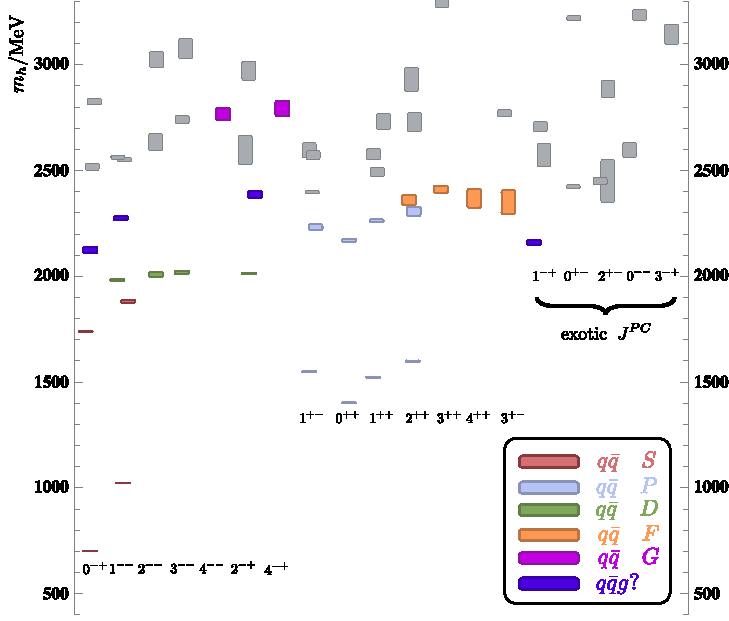
\includegraphics[width=\linewidth]{figures/LatticeSpectrum743/SpinAndWaveIdentAll.pdf}
\caption{ Here we present a lattice calculation where we have identified the spin, parity, and charge conjugation quantum numbers for a variety of states. Boxes represent energy levels extracted in our calculation, the size of the box corresponding to the uncertainty of the extracted energy. Different supermultiplet candidate states are grouped according to color. This calculation was performed in a version of QCD with three flavors of quarks all tuned to approximately the strange quark mass, further details of the lattices can be found in \secref{sec::res::calc_det}. \label{fig::MultipletIdent743Spec}}
\end{centering}
\end{figure}
\clearpage
}
%%%%%%%%%%%%%%%%%%%%%%%%%%%%%%%%%%%%%%%%%%%%%%%%%%%%%%%%%
%%%%%%%%%%%%%%%%%%%%%%%%%%%%%%%%%%%%%%%%%%%%%%%%%%%%%%%%%
%%%%%%%%%%%%%%%%%%%%%%%%%%%%%%%%%%%%%%%%%%%%%%%%%%%%%%%%%






